\documentclass[runningheads,a4paper]{llncs}

\usepackage{amssymb}
\setcounter{tocdepth}{3}
\usepackage{graphicx}
\usepackage{calc,listings,color}

\usepackage[ruled,nothing]{algorithm}
\usepackage{algorithmic}
\renewcommand{\algorithmicrequire}{{\textbf{Input:}}}
\renewcommand{\algorithmicensure}{{\textbf{Output:}}}

\usepackage{url,xspace}

\newcommand{\linbox}{{\sc LinBox}\xspace}

\begin{document}

\mainmatter  
\title{\linbox founding scope allocation, parallel building blocks, and
  separate compilation}
\titlerunning{\linbox memory, parallelism, compilation models}

\urldef\jgdemail\url{Jean-Guillaume.Dumas@imag.fr}
\urldef\cpemail\url{Clement.Pernet@imag.fr}
\urldef\bdsemail\url{saunders@udel.edu}
\urldef\tgemail\url{Thierry.Gautier@inrialpes.fr}

\author{
Jean-Guillaume Dumas\inst{1}
\and Thierry Gautier\inst{2}
\and Cl\'ement Pernet\inst{2}
\and B. David Saunders\inst{3}
}
\authorrunning{J-G. Dumas, T. Gautier, C.
  Pernet, B. D. Saunders}

\institute{
Laboratoire J. Kuntzmann, Universit\'e de
Grenoble. 51, rue des Math\'ematiques, umr CNRS 5224, bp 53X, 
F38041 Grenoble, France, \jgdemail.
\and
Laboratoire LIG, Universit\'e de Grenoble. umr CNRS, 
F38330 Montbonnot, France. \cpemail, \tgemail.
\and University of Delaware, Computer and
  Information Science Department. 
Newark / DE / 19716, USA. \bdsemail.}

\maketitle

\section{Introduction}

As a building block for a wide range of applications, computational exact linear
algebra has to conciliate both efficiency and genericity. The goal of the 
\linbox project is to address this problem by designing an efficient general-purpose
\texttt{C++} open-source library for exact linear algebra over the integers, the
rationals and finite fields. 
Matrices can be either dense, sparse or black box (i.e. viewed as a linear
operator, acting on vectors only). The library proposes a set of high level
linear algebra solutions, such as the rank, the determinant, the solution of a
linear system, the smith normal form, the echelon form, the characteristic
polynomial, ... Each of these solutions involve a hybrid combination of several specialized
algorithms depending on the domain, and the type of matrix. Over a finite field,
the building blocks are an efficient implementation of Wiedemann and block
Wiedemann algorithms combined with preconditioners~\cite{CEKSTV:2002:EP} for
black box matrices, a sparse Gaussian elimination for sparse matrices and the
BLAS based dense linear algebra techniques of the \texttt{FFLAS}
library~\cite{DGP:2008:dlaff} for dense matrices. The solutions over the integers
and rationals are lifted from modular computations by a Chinese remainder
algorithm or $p$-adic lifting.
The design based on a high genericity allow to write efficient algorithms  independently from the
representations of domains and matrices. As a middleware, the library relies on the
efficiency of kernel libraries such as  \texttt{GMP}\footnote{\url{http://gmplib.org/}},
\texttt{Givaro}\footnote{\url{http://www-ljk.imag.fr/CASYS/LOGICIELS/givaro/}},
\texttt{NTL}\footnote{\url{http://www.shoup.net/ntl/}},
\texttt{ATLAS}\footnote{\url{http://math-atlas.sourceforge.net/}} and can be used by general
purpose computer algebra systems such as \texttt{Sage}\footnote{\url{http://sagemath.org/}} or \texttt{Maple}\footnote{\url{http://www.maplesoft.com/}}. 

We describe in this paper a selection of ideas and
improvements that were recently introduced into the the design of LinBox 
for the forthcoming major release v2.0.

\section{A lightweight memory management model}

%\subsection{Call-by-reference}

The main objects that require memory allocation in \linbox are base field or
ring elements, vectors, matrices, and polynomials.
The memory management for all of these object types follows the same rules, organized to
maximize efficiency in time and space, and consequently requiring some
efforts by  the programmer. In particular no external garbage collection
mechanism is used.

The input and output types of most functions are usually template
types, and can be either basic types, or complicated
objects. Consequently, passing arguments by value (copy) must be avoided as
much as possible. Every argument is passed as a reference, including
the return types. More precisely the return value of a function is
also the first argument, defined as a non const reference. 

\begin{verbatim}
Matrix & someFunction( Matrix & result, const XXX& args);
\end{verbatim}

This convention was already presented in \cite[\S 2.1]{jgd:2002:icms} for the
design of field and ring arithmetic. It does require a redefinition of the interface
for some \texttt{stl}-like operators, as discussed in
section~\ref{ssec:parallel}.

\subsection{The founding scope allocation model}

A consequence of the above convention is that the objects returned by
a function,
have to be declared and initialized (in particular, memory allocated) (e.g. via constructors) before the
function call.
By enforcing this
practice, we require that the programmer keep 
\textit{the handle} on the
objects that he allocates until all uses of the object and it's subobjects are completed. Moreover, he is responsible for object 
deallocation in the same 
scope where it was allocated. 
This restricts some convenient programming practices, but provides precise control of memory usage.
This is particularly important when large, memory filling, matrices
are in play.
It also allows to avoid the costs of garbage 
collection or reference counting.

Many LinBox objects involve a handle containing a reference to the free store.
Note that even though a function does not allocate the return value handle,
it is in some cases still free to resize and thus reallocate the free store memory referenced.


\begin{paragraph}{Dense Matrix allocations.}
The objects representing dense matrices require a special care concerning  their
allocations. Dense matrices are stored as a one dimensional array storing
elements in the row major format : \texttt{A[i,j] = *(A+i*n+j)}. It is important
to be 
able to define a submatrix as a view on such an array, without allocating the
data. Thus a first approach is to define a dense matrix class with a
boolean \texttt{\_alloc} 
member, telling whether the matrix owns its data or whether it is a simple  view
on some other matrix's data. The destructor deallocates the data only if
\texttt{\_alloc} is \texttt{true}. This can be viewed as a simplified
reference 
counting mechanism, where one assumes that the matrix initially allocated is
always destructed after all of its sub-matrices. This convention is consistent
with the previous consideration: the allocations and deallocations must always
occur in the founding scope.

To further improve the efficiency, an alternative is to distinguish
two classes: 
one for allocated matrices and the other for sub-matrix views. The
genericty of 
 the template mechanism or inheritance will allow to use these two
 types in the same code, without duplication. Furthermore,
 thread-safety mechanism on the \texttt{\_alloc} 
member are not required anymore.
\end{paragraph}
% It's clear we haven't resolved this!
% I would argue that the founding scope model (mother model) implies that 
% neither the alloc variable nor a 2 classes system is required.  
% The programmer knows whether a matrix is created as a submatrix 
% or as an allocating instance by what constructors or other initializers 
% she uses.  Thus she knows which require care to deallocate in the same scope. 
% What she doesn't necessarily get is automatic decision about delete 
% in the destructor, may have to call an explicit "end of use" function 
% to get the delete.  
% So: 1) 2 class system requires an extra explicit declaration of base object.
%	  2) alternative is to require programmer to make explicit "end of use" call on base (allocating) objects.
%      3) alloc allows to require neither of the programmer.

\begin{paragraph}{Rebind of matrices.}
We illustrate the founding scope allocation model with the use of rebind
functions adapted from the allocators in the STL.
\linbox makes use of the concept of rebinds for the mapping of data
structures between different coefficient domains.
For instance, in the context of the Chinese remainder algorithm rebinds
allow to map a matrix over the integers of type, say,
(\texttt{DenseMatrix<PID\_Integer>}) to a modular matrix of type, say,
(\texttt{DenseMatrix<Modular<double> >}).
\begin{verbatim}
template <class Domain>
class DenseMatrix {
  typedef DenseMatrix<Domain> Self_t;
  ... 
  template<class AnyDomain>
  struct rebind{ 
     typedef DenseMatrix <AnyDomain> other;
     operator ()(other& Ap, const Self_t& A, const AnyDomain& D){
       // Performs the modular conversion of A to Ap over D
       ...
     } 
  };  
}
\end{verbatim}

According to the founding scope allocation model, the function
\texttt{operator()} in charge of the initialization of the matrix cannot 
allocate any memory. This has to be done at the level where the
rebind is called. This also requires a modification of the rebind
operator interface of the STL: the new object is passed by reference.

In \linbox, these binder adaptors are enclosed
within many data structure and make use of a generic
converter, named \texttt{Hom} and found in \url{linbox/field/hom.h}.
Indeed, \texttt{Hom} can generically use the \linbox domain's canonical
convertion methods methods \url{init} and \url{convert} to the \linbox
Integer type: \texttt{Domain} $\rightarrow$ \texttt{Integer}
$\rightarrow$ \texttt{AnyDomain}. 
Moreover, when natural convertions exists between domains's
(e.g. different representations of the same field or embedded domains,
...) this can be directly bypassed by a specilization of \texttt{Hom}.
\end{paragraph}

Overall, the founding scope allocation model is quite natural (the caller is
solely responsible for the physical construction/destruction) and very
efficient: memory is allocated a minimal number of times and
automatically freed by the destructor mechanism. Moreover, thread
safety is facilitated: memory is handled within the scope of the
caller, and thus by the allocating thread. % I don't buy this last sentence.

\section{Software abstraction layer for parallelism}

Efficient parallel applications must take into consideration hardware
characteristics (number of cores, memory hierarchy, etc.). It is time
consuming or impossible for a single developer to 
program a high performance computer algebra application, with state of
the art algorithms, while exploiting all the available parallelism.  
In order to separate the domains of expertise we have designed a
software abstraction layer between computer algebra algorithms
and parallel implementations which may employ automatic dynamic scheduling.

\subsection{Parallel building blocks}\label{ssec:parallel}
Computer algebra algorithms have three main characteristics:
\begin{enumerate}
\item They are complex and require a deep knowledge of the problem in
  order to the most efficient sequential algorithm.
\item They may be highly irregular. This enforces a runtime use of
  load balancing algorithms.
\item They are generic in the sense that it they are usually designed
  to work over several algebraic domains.
\end{enumerate}

  In the case of \linbox algorithms, we have decided to base our
  software abstraction, called {\em Parallel Building Blocks (PBB)},
  on the STL algorithms (Standard Template Like) principles.

  Indeed, C++ data structures in \linbox let us to have random access
  iterators over containers which are naturally parallel. 
  
  We have already defined several STL-like algorithms and the list
  will be extended in the near future:
  \begin{description} 
    
  \item [for\_each, transform, accumulate \cite{Musser:1996:STL}:] the PBB
    versions of these three algorithms are similar to the STL versions 
    except that the involved operators (or function object classes) given as 
    parameters are required to have their return value reference passed as the
    first parameter of the function in accordance with the memory model 
	of \linbox. 
    The STL return-by-value semantic is not appropriate. 
  \end{description} 
  
  Note that within the emerging C++0x standard, the lambda capability
  of the core language will simplify the use of these operators and
  therefore of the parallel building blocks.

%\verb!transform!, etc. 

%\begin{itemize}
%\item Transparent parallelism
%\item Abstraction of parallelism
%\item Parallelism really as a plug-in
%\end{itemize}
  
  The fundamental idea of these blocks is that at the computer algebra
  level, the parallelization of all the loops and more generally of all
  the STL-like algorithms will already enable:
\begin{enumerate}
\item Good performance: in many complex or irregular computer algebra
  applications this coarse-grain parallelization of the inner loops of
  the underlying linear algebra is sufficiently refined.
\item Multiple implementations of the parallel blocks: this
  abstraction allows for both a programming independent of the
  parallel model and a selection of the parallel environment
  depending on the target architecture.
\end{enumerate}

The parallel blocks can be implemented using many different parallel
environments, such as OpenMP
\cite{Chapman:2007:openmp}; TBB (Thread Building Blocks)
  \footnote{\url{http://www.threadingbuildingblocks.org}} or
  Kaapi~\cite{inproceedingsgautier.gbp_ktsrsf_07}; using
  both static or dynamic work-stealing
  schedulers~\cite{con-traore.trmgb_08}.
The current implementations are built on OpenMP and Kaapi.

\subsection{Accumulate-while and early termination}
To bound the complexity of many linear algebra problems, one of the
key idea is to use an accumulation with {\em early termination}.

For instance, this is used in Chinese Remaindering algorithms. The
computation is performed modulo a sequence of (co)prime numbers and
the result is built from a sequence of residues, {\em only while} a
condition is satisfied~\cite{jgd:2010:crt}. 
The termination of the algorithm depend on the accumulated (here
reconstructed) result.
  
In order to parallelize such algorithms, we proposed an extension of
the STL algorithms called \verb+accumulate_while+:
\begin{description} 
\item [accumulate\_while:] The algorithm takes an array $v$ of length $N$, a unary
  operator $f$ to be applied to each array entry, a binary operator $+$ for the accumulation, and a predicate
  operator (giving the termination condition).
  Let $S_k = \sum_{i=0,..,k} f( v[i])$ with 
  $k \in \{0,N\}$, the algorithm computes and returns $n \leq N$ and $S_n$ such that 
  $S_k, k \leq n$ may not satisfy the predicate and either $n = N$ or $S_n$
  does satisfy the condition.
\end{description} 

  This algorithm will be used 
  for the early termination Chinese remaindering algorithms of
  \linbox. Though not yet using PBB and accumulate_while, a sequential version and parallel versions with OpenMP and
  Kaapi can be found in the \linbox distributions as 
  \url{linbox/algorithms/cra-domain-*.h}.

%\verb!Accumulate-while!, generalization of \cite{jgd:2010:crt},
%specially adapted to early termination in mathematical softwares.
%Other applications (e.g. from \cite{Beaumont:2004:PMAA}) ??


\subsection{Memory contention and thread safe allocation}
Many computer algebra programs allocate dynamic memory for the
intermediate computations. Several experiments with \linbox
algorithms, on multicore architectures, have shown that these
allocations are quite often the bottleneck in the performance.

An analysis of the memory pattern and experiments with three well
known memory allocators 
(ptmalloc, Hoard and TCMalloc from Google Perf. Tools~\cite{tcmalloc})
have been conducted. The goal was to decide whether the parallel
building blocks model was suitable to high-performance exact linear
algebra. We used dynamic libraries to exchange allocators for the
experiments, but one can use them together in the \linbox library if
needed \cite[\S 7]{kaltofen:2005:memory}.

Preliminary experiments on the Chinese remaindering {\bf accumulate\_while},
not the easiest to parallelize, have demonstrated the advantage, in
our setting, of TCMalloc over the others~\cite{jgd:2010:crt}.
One of the main reason for that fact is that our problems required
many temporary allocations. This fits precisely the thread safe caching
mechanism of TCMalloc.

\section{Automated Generic Separate compilation}
\linbox is developed with several levels of genericity:
\begin{itemize}
\item Genericity with respect to the domain of the coefficients;
\item Genericity with respect to the data structure of the matrices;
\item Genericity with the intermediate algorithms;
\item ...
\end{itemize}
While efficient in terms of capabilities and code reusability, this
can lengthen the compilation time and generate large executable files.\\
For the management of code bloat \linbox proposes an ``archetype
mechanism'' which enable, at the user latitude, to switch to a
compilation against abstract classes \cite[\S 2.1]{jgd:2002:icms}.\\
This can reduce the efficiency of the library. Therefore, we propose
here a way to provide a generic separate compilation. This will not
deal with code bloat, but will reduce the compilation time while
preserving the performances.\\
This is useful for instance when the library is used with
unspecialized calls. This is largely the case for some interface
wrappers to other Computer algebra systems such as {\sc Sage} or {\sc Maple}.\\
Our idea is to automatize the technique of
\cite{Erlingsson:1996:issac} which combines compile-time instantiation
and link-time instantiation, while using template instantiation
instead of void pointers.\\
The mechanism we propose is independent of the desired generic method,
candidate
for separate compilation, and is explained on algorithm \ref{alg:sep}.
\begin{algorithm}[ht]
\caption{C++ Automatic separate compilation wrapping}\label{alg:sep}
\begin{algorithmic}[1]
\REQUIRE A generic function \texttt{func}.
\REQUIRE Some template parameters for separate specialization and
compilation of  \texttt{func}.
\ENSURE A generic function calling
\texttt{func} with separately compiled instantiations.
\STATE Create a header and a body files ``func\_instantiate.hpp'' and ``func\_instantiate.cpp'';
\STATE Add a template function \texttt{func\_separate}, with the same
specification as \texttt{func}, to the header;
\STATE Its generic default implementation is a single line calling the
original function \texttt{func}.\\ \COMMENT{This enables to have a
  unified interface, even for non specialized class.}
\FOR{each separately compiled template parameter \texttt{TParam}}
  \STATE Add  a non template specification
  \texttt{funcTParam}, to the header file;
  \STATE Add the associated body with a
  single line returning the instantiation of
  \texttt{func} on a parameter of type \texttt{TParam}, to the body file;
  \STATE Add an inline specialization
  body of \texttt{func\_separate} on a parameter of type
  \texttt{TParam} with a single line returning \texttt{funcTParam}, to
  the header file; 
\ENDFOR
\STATE Compile the body file ``func\_instantiate.cpp''.
\end{algorithmic}
\end{algorithm}

This Algorithm is illustrated on figure \ref{fig:sep}, where
the function is the \texttt{rank} and the template parameter is a dense
matrix over the finite field with two elements,
\texttt{DenseMatrix<GF2>}.
\begin{figure}[ht]
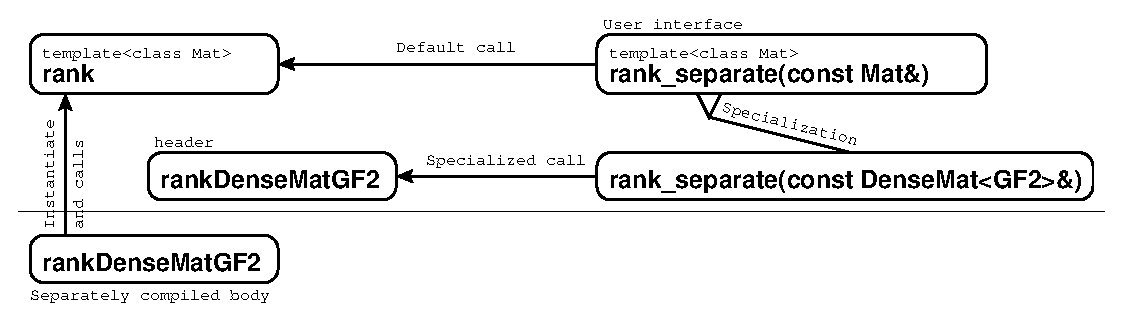
\includegraphics[width=\textwidth]{separate}
\caption{Separate compilation of a rank specialization}\label{fig:sep}
\end{figure}

%
\begin{remark} Algorithm \ref{alg:sep} has been simplified for the
  sake of clarity. To enable a more user-friendly interface and to
  leave it unchanged, one can rename the original function and all its
  original specializations \texttt{func\_original}; then rename also
  the new interface (\texttt{func\_separate}) simply
  \texttt{func}. This allows to keep the legacy
  interface unchanged. 
\end{remark}

\begin{remark} 
With the classical inline compiler optimizations, the overhead of
calling \texttt{rank\_separate} is limited to single supplementary
function call. Indeed all the one line additional methods will be
automatically inlined, except, of course, the one calling the separately
compiled code.
If this overhead is nonetheless too expensive, it suffices to enclose all the non generic specializations of
``func\_instantiate.hpp'' by a macro test. 
At compile time, the decision to separately
compile or not can be taken according to the definition of this
macro. 
\end{remark}


We show on table \ref{tab:compilation} the gains, in term of compilation time,
obtained on two examples of \linbox: the \texttt{examples/rank.C} and
\texttt{examples/solve.C} algorithms. Indeed without any specification
the code
has to be generic and to invoke several specializations depending on
run-time discovered properties of the input. For instance the
\texttt{solve.C} example requires at least 6 specializations for sparse
matrices over the Integers or over a prime field, with a sparse
elimination, or an iterative method, or a dense method if the matrix
is small, or an hybrid method...
\begin{table}[ht]\center
\begin{tabular}{|l||r|r|r||r|r|r|}
\hline
file                      &  real time   &  user time   &  sys. time  &  real time   &  user time   &  sys. time \\
\hline
 & \multicolumn{3}{|c||}{Rank}& \multicolumn{3}{|c|}{Solve}\\
\hline
\texttt{instantiate.o} & 143.43s & 142.47s & 0.90s & 171.62s & 170.42s & 1.12s\\
\texttt{\{rank,solve\}.o} & \bf 18.58s & \bf 18.26s & \bf 0.30s & \bf 23.13s & \bf 22.80s & \bf 0.32s\\
\texttt{link} & 0.80s & 0.64s & 0.15s & 0.85s & 0.70s & 0.14s\\
\hline
\texttt{Sep. comp. total} & 162.81s & 161.37s & 1.35s & 195.60s & 193.92s & 1.58s\\
\hline
\texttt{Full comp.} & 162.02s & 160.47s & 1.21s & 191.47s & 189.52s & 1.40s\\
\hline
\hline
\texttt{speed-up} & 8.4 & 8.5 & 2.7 & 8.0 & 8.1 & 3.0s\\
\hline
\end{tabular} 
\caption{linbox/examples/\{rank,solve\}.C compilation time on an AMD
  Athlon 3600+, 1.9GHz, with gcc 4.5 -O2. \texttt{instantiate.o} corresponds to the separately compiled
  instantiations (e.g. densegf2rank in figure \ref{fig:sep});
  \texttt{\{rank,solve\}.o} corresponds to the user interface and generic
  implementation compilation; \texttt{link} corresponds to the
  linking of both \texttt{.o} and the library; \texttt{Full comp.}
  corresponds to the compilation without the separate
  mechanism.}\label{tab:compilation}
\end{table}

\section*{Acknowledgment}
We thank the \linbox group and especially Brice Boyer, Pascal Giorgi,
Erich Kaltofen, Dan Roche, Brian Youse for many useful discussions 
in particular during the recent \linbox developer meetings in
Delaware and Dublin.

\bibliographystyle{plain}
\bibliography{icms} 

\end{document}
